\documentclass[11pt]{article}

\usepackage[T1]{fontenc}
\usepackage[margin=1in]{geometry}
\usepackage{amsmath,amssymb}
\usepackage{booktabs}
\usepackage{float}
\usepackage{graphicx}
\usepackage{microtype}
\usepackage[numbers,sort&compress]{natbib}
\usepackage{xcolor}
\usepackage{xspace}
\usepackage[hidelinks]{hyperref}

\graphicspath{{figures/}}

\newcommand{\method}{\textsc{EFF-Dock}\xspace}
\newcommand{\angstrom}{\text{\normalfont\AA}}
\newcommand{\R}{\mathbb{R}}
\newcommand{\SO}{\mathrm{SO}}
\newcommand{\SE}{\mathrm{SE}}
\newcommand{\todo}[1]{\textcolor{red}{[TODO: #1]}}

\title{\method: Fragment-Based \(\SE(3)\)-Equivariant Flow Matching\\
for Protein--Ligand Docking}
\author{\parbox{0.96\textwidth}{\centering
Jaemin Sim\textsuperscript{1} and
Juyong Lee\textsuperscript{1,2,3,4,*}\\[0.75em]
\small\textsuperscript{1}Department of Molecular Medicine and
Biopharmaceutical Sciences, Graduate School of Convergence Science and
Technology, Seoul National University, Seoul 08826, Republic of Korea\\
\small\textsuperscript{2}College of Pharmacy, Seoul National University,
Seoul 08826, Republic of Korea\\
\small\textsuperscript{3}Research Institute of Pharmaceutical Science,
College of Pharmacy, Seoul National University, Seoul 08826,
Republic of Korea\\
\small\textsuperscript{4}Arontier Co., Seoul 06735, Republic of Korea\\[0.5em]
\small\textsuperscript{*}Corresponding author:
\href{mailto:nicole23@snu.ac.kr}{nicole23@snu.ac.kr}
}}
\date{}

\begin{document}

\maketitle

\begin{abstract}
Protein--ligand docking requires sampling multimodal poses while preserving
ligand geometry and three-dimensional equivariance. We introduce \method, a
fragment-based \(\SE(3)\)-equivariant flow-matching model that transports
connected rigid fragments from a pocket-centered prior to a bound pose and
uses a Newton--Euler readout to convert atom-level equivariant predictions
into fragment translation and angular velocities. A separate confidence
network ranks 80 generated candidates without modifying the docking
generator. In a frozen reference-pocket redocking diagnostic, pure-confidence
top-1 selection achieves symmetry-aware heavy-atom RMSD below
\(2\,\angstrom\) for 76.47\% of Astex Diverse, 73.05\% of PoseBusters v2, and
69.47\% of CASF-2016 complexes, while oracle-80 coverage ranges from 91.93\%
to 95.29\%. These results separate candidate generation, pose selection, and
physical validity, but do not constitute blind-pocket, apo-receptor, or
prospective docking evidence.

\end{abstract}

\noindent\textbf{Keywords:}
protein--ligand docking; flow matching; equivariant neural network;
molecular fragmentation; pose confidence

\section{Introduction}
\label{sec:introduction}

The three-dimensional pose of a small molecule determines which chemical
groups can contact a protein, which interactions can be formed, and which
modifications are sterically accessible. Reliable complex structures therefore
support the interpretation of structure--activity relationships, selectivity,
and resistance mutations, and provide starting hypotheses for medicinal
chemistry and more expensive physics-based calculations. Experimental complex
structures remain costly and incomplete, however, particularly for new targets
and ligand series. Protein--ligand docking addresses this gap by predicting a
ligand pose conditioned on a receptor structure and, in the setting considered
here, a specified binding site. This is a geometric prediction problem:
recovering a plausible pose is important for structure-based design, but a
docking score or pose-confidence score is not by itself a binding-affinity
measurement.

Docking is difficult because ligand placement and internal conformation are
strongly coupled. A candidate must resolve global translation and orientation,
multiple rotatable bonds, local protein--ligand complementarity, and
intramolecular geometry on a rugged, multimodal landscape. Protein motion,
uncertain protonation and tautomeric states, cofactors, metals, and solvent can
further change the relevant interaction pattern. Classical docking programs
combine a conformational search with an approximate scoring function and have
become indispensable, practical tools \citep{trott2010vina}; nevertheless,
tractable search often requires a rigid or only locally flexible receptor.
Ligand-induced conformational changes can consequently create a substantial
gap between docking into an available apo structure and redocking into the
experimental holo structure \citep{lu2024dynamicbind}.

Deep generative models have recently changed the formulation of the problem.
DiffDock casts ligand docking as diffusion over translational, rotational, and
torsional degrees of freedom and samples multiple candidate poses
\citep{corso2023diffdock}. DynamicBind extends geometric generation toward
ligand-specific receptor conformations \citep{lu2024dynamicbind}, while
AlphaFold~3 demonstrates that raw all-atom coordinates of proteins, ligands,
nucleic acids, ions, and modified residues can be generated in a unified
cofolding framework \citep{abramson2024alphafold3}. In parallel, FlowDock
applies conditional geometric flow matching to flexible protein--ligand
complex generation \citep{morehead2025flowdock}. Collectively, these results
show that learned generative vector fields can explore complex pose
distributions without relying exclusively on hand-designed search heuristics.
They also make the distinction between tasks more important: blind cofolding
from sequence, docking into a predicted apo receptor, known-pocket docking,
and reference-pocket holo redocking expose models to different information and
should not be compared as if they were the same prediction problem.

Despite this progress, three limitations remain central. First, sampling and
selection are different problems. A generator may place a near-native pose
among many samples while its confidence model fails to rank that pose first.
Second, coordinate accuracy and molecular validity are different axes:
low heavy-atom RMSD does not ensure valid stereochemistry, bond geometry, or
absence of severe clashes \citep{buttenschoen2024posebusters}. Third, random
row-level splits can overstate generalization when related ligands, homologous
pockets, or alternate structures cross the train--test boundary. Recent
systematic studies have found that performance changes materially for predicted
apo receptors, unknown pockets, multiligand systems, and previously unseen
protein--ligand poses \citep{morehead2026posebench}. A post-training-cutoff
study of 2,600 high-resolution systems further reported strong dependence of
cofolding accuracy on similarity to training examples
\citep{skrinjar2026generalization}. These observations motivate
similarity-aware resources such as PLINDER \citep{durairaj2024plinder} and
require every docking result to declare the receptor state, pocket
information, sampling budget, ranking rule, and leakage boundary.

The representation used for ligand flexibility is another consequential
choice. Treating the entire ligand as one rigid body preserves chemistry but
cannot express torsional rearrangement. Directly generating every atom is
maximally flexible, but requires the model to maintain covalent geometry while
solving the global docking problem. Torsion-based models preserve bond lengths
and angles, yet a rotation about one bond moves an entire downstream subgraph
and ties the parameterization to a particular molecular-tree convention. We
instead use rigid fragments as an intermediate geometric scale. Rotatable bonds
partition the ligand into locally rigid components, and the pose is represented
by one translation in \(\R^3\) and one proper rotation in \(\SO(3)\) per
fragment. This factorization preserves internal fragment geometry while
allowing cooperative relative motion across flexible bonds. Because independent
fragment poses can strain the cut-bond interfaces, the representation must be
paired with explicit fragment adjacency, cross-fragment geometry, and
atom-level contact reasoning.

We introduce \method for pocket-conditioned protein--ligand docking. It uses
fragment-based \(\SE(3)\)-equivariant flow matching. Given a receptor
structure, ligand graph, and externally supplied pocket center,
\method crops a \(10\,\angstrom\) receptor neighborhood and constructs a
heterogeneous graph of ligand atoms, ligand fragments, protein atoms, and
residue nodes. A shared equivariant trunk communicates through covalent,
fragment, residue, and dynamically rebuilt protein--ligand contact edges. The
network predicts equivariant atom-level force-like vectors and aggregates them
into fragment translations and angular velocities through a Newton--Euler
construction. Flow matching learns the time-dependent vector field that
transports independently sampled fragment poses toward the bound pose, while a
separately trained confidence model ranks the resulting candidate set. The
receptor is fixed, and the model neither discovers an unknown pocket nor
predicts binding affinity; this deliberately narrow contract permits a precise
assessment of pose generation and selection.

Our main contributions are:
\begin{itemize}
    \item We formulate flexible ligand docking as flow matching on a product of
    fragment rigid-body pose spaces and introduce an atom-to-fragment
    Newton--Euler head that preserves \(\SE(3)\) equivariance while coupling
    local contact evidence to global fragment motion.

    \item We develop a unified heterogeneous interaction network with
    higher-order irreducible representations, time conditioning, explicit
    cross-fragment geometry, and dynamic protein--ligand contacts, together
    with a matched confidence model for top-1 pose selection.

    \item We separate sampling coverage, deployable selection, and physical
    validity in evaluation. On frozen \(10\,\angstrom\) reference-pocket
    redocking manifests for Astex Diverse and PoseBusters v2, we
    compare the first sample, score-based and learned selectors, and an
    explicitly non-deployable best-of-80 oracle under the same candidate sets.

    \item We state the scientific boundary of the current evidence: the
    reported benchmark is a compatibility diagnostic with target-derived
    pocket centers, not a claim of blind docking, affinity prediction, or
    prospective chemical and pocket generalization. This makes the remaining
    strict-split retraining and apo-receptor tests explicit rather than
    conflating them with holo redocking performance.
\end{itemize}

\section{Method}
\label{sec:method}

\subsection{Problem formulation}

The prediction unit is one receptor structure, one ligand chemical entity, and
one explicitly specified binding pocket. The model receives receptor
coordinates and atom/residue identities, the ligand molecular graph and
stereochemistry, and a pocket center. It does not receive the crystallographic
ligand coordinates, pose RMSD, benchmark identity, or any feature computed
from a downstream evaluation. The output is a set of sampled all-atom ligand
poses and a separately declared pose-selection score. \method is a pose
generator and ranker; it is not trained as an affinity predictor or a blind
pocket detector.

Let the ligand contain \(N\) heavy atoms partitioned into \(K\) rigid
fragments. Atom \(i\) has a fragment assignment \(g(i)\) and a fixed
fragment-local coordinate \(\mathbf{y}_i\). A ligand pose is parameterized by
one translation and one proper rotation per fragment,
\[
    \mathbf{z}
    =
    \left\{(\mathbf{T}_k,\mathbf{R}_k)
    \mid \mathbf{T}_k\in\R^3,\,
    \mathbf{R}_k\in\SO(3)\right\}_{k=1}^{K},
\]
and the corresponding global atom coordinate is
\begin{equation}
    \mathbf{x}_i
    =
    \mathbf{R}_{g(i)}\mathbf{y}_i+\mathbf{T}_{g(i)}.
    \label{eq:atom_reconstruction}
\end{equation}
This representation preserves the internal geometry of each fragment while
allowing relative fragment motions to express ligand flexibility.

\subsection{Rigid-fragment decomposition}
\label{sec:fragmentation}

Ligands are sanitized and featurized with RDKit
\citep{landrum2024rdkit}. We identify cuttable bonds as heavy-atom single
bonds that are outside rings, are not planar conjugated bonds such as
amide-like linkages, and have endpoints with heavy-atom degree greater than
one. Candidate bonds are processed in deterministic order. A cut is accepted
only when each endpoint retains at least one non-cut heavy-atom bond, which
prevents isolated atoms along simple chains. Any remaining singleton component
is merged into its largest adjacent fragment. The resulting connected
components define \(g(i)\).

For each retained cut bond, we preserve the fragment adjacency and add local
cross-fragment triangulation edges around the cut-bond atoms. Their reference
distances provide a geometry signal without fixing the torsion angle. Fragment
centers are the geometric means of their member atoms, and local coordinates
are formed by subtracting the corresponding center. Single-atom fragments,
when unavoidable, have no supervised rotational degree of freedom.

\begin{figure}[t]
    \centering
    
\includegraphics[width=\textwidth]{fragmentation_examples.png}
    \caption{Rigid-fragment representation. Cuttable rotatable bonds are
    highlighted in red, and atoms belonging to the same connected rigid
    component share a color. The model predicts one translation and one proper
    rotation per retained fragment while preserving atom-level chemistry and
    fragment adjacency.}
    \label{fig:fragmentation}
\end{figure}

\subsection{Pocket-conditioned heterogeneous graph}
\label{sec:graph}

The receptor is cropped in a residue-aware manner around the supplied pocket
center. During training, the current configuration samples the crop radius
uniformly from \(6\) to \(12\,\angstrom\) and applies Gaussian center jitter
with standard deviation \(2\,\angstrom\). The matched confidence and external
redocking protocol uses a fixed \(10\,\angstrom\) crop without center jitter.
At prospective inference, the pocket center must be supplied independently of
the unknown target pose.

We construct a single heterogeneous graph with four node types:
ligand atoms, ligand fragments, protein atoms, and protein-residue virtual
nodes. Ligand atom features encode element, formal charge, aromaticity,
hybridization, valence, chirality, ring membership, and pharmacophore flags.
Protein atom features encode residue--atom identity, backbone and metal
indicators, and protein-side pharmacophore flags. Residue virtual nodes encode
residue identity and provide a coarser structural communication path.

Ten typed edge relations represent ligand covalent bonds, local
triangulation, cut bonds, atom-to-fragment ownership, fragment adjacency,
protein covalent bonds, atom-to-residue membership, residue connectivity,
residue-to-fragment context, and dynamic protein-to-ligand contacts.
At flow time \(t\), the graph is
\(\mathcal{G}_t=(\mathcal{V},\mathcal{E}_{\mathrm{static}}\cup
\mathcal{E}_{\mathrm{contact},t})\). Protein--ligand atom contact edges are
rebuilt bidirectionally at every forward pass:
\begin{equation}
    \mathcal{E}_{\mathrm{contact},t}
    =
    \left\{
    (p,i),(i,p)
    \,\middle|\,
    p\in\mathcal{V}_{\mathrm{prot\text{-}atom}},
    i\in\mathcal{V}_{\mathrm{lig\text{-}atom}},
    \|\mathbf{x}_{p}-\mathbf{x}_{i,t}\|_2\leq 5\,\angstrom
    \right\}.
    \label{eq:dynamic_contacts}
\end{equation}
Edges are created only within the same complex in a minibatch.

For an edge \(j\rightarrow i\), define
\(\mathbf{r}_{ji}=\mathbf{x}_i-\mathbf{x}_j\) and
\(d_{ji}=\|\mathbf{r}_{ji}\|_2\). Edge attributes combine a 32-component
radial basis expansion with relation, bond, fragment-topology, local-frame,
pair-chemistry, endpoint-state, and time features. Their exact construction is
given in Appendix~\ref{app:edge_features}.

\subsection{Flow matching on fragment poses}
\label{sec:flow}

We center coordinates at the pocket and define a factorized prior over
fragment poses. For each fragment \(k\),
\begin{equation}
    \mathbf{T}_{k,0}
    \sim
    \mathcal{N}(\mathbf{0},\sigma^2\mathbf{I}),
    \qquad
    \mathbf{R}_{k,0}
    \sim
    \mathrm{Uniform}(\SO(3)).
    \label{eq:pose_prior}
\end{equation}
Single-atom fragment rotations are fixed to identity. During training,
\(\sigma\in\{0.5,1,2,3,4\}\,\angstrom\) is sampled with probabilities
\(\{0.10,0.25,0.30,0.25,0.10\}\), and \(\log\sigma\) is embedded along with
time. A global random proper rotation is applied to the ligand representation
as augmentation.

Given prior and target fragment poses
\((\mathbf{T}_{k,0},\mathbf{R}_{k,0})\) and
\((\mathbf{T}_{k,1},\mathbf{R}_{k,1})\), respectively, the default objective
uses a linear translation path and shortest-path spherical interpolation for
rotation:
\begin{align}
    \mathbf{T}_{k,t}
    &=
    (1-t)\mathbf{T}_{k,0}
    +t\mathbf{T}_{k,1},
    \label{eq:translation_path}\\
    \mathbf{R}_{k,t}
    &=
    \operatorname{Exp}(t\boldsymbol{\omega}^{\star}_k)
    \mathbf{R}_{k,0},
    \label{eq:rotation_path}\\
    \boldsymbol{\omega}^{\star}_k
    &=
    \operatorname{Log}
    \left(\mathbf{R}_{k,1}\mathbf{R}_{k,0}^{-1}\right).
\end{align}
The world-frame conditional velocity targets are therefore
\begin{equation}
    \mathbf{v}^{\star}_k
    =
    \mathbf{T}_{k,1}-\mathbf{T}_{k,0},
    \qquad
    \boldsymbol{\omega}^{\star}_k
    =
    \operatorname{Log}
    \left(\mathbf{R}_{k,1}\mathbf{R}_{k,0}^{-1}\right).
    \label{eq:flow_targets}
\end{equation}
Following the flow-matching formulation \citep{lipman2023flow}, a time-
conditioned network regresses these vector fields without integrating an ODE
during training. Time is sampled from
\[
  p(t)=0.02\,\mathcal{U}(0,1)
  +0.98\,\operatorname{sigmoid}
  \left(\mathcal{N}(0.8,1.7^2)\right),
\]
which emphasizes late refinement while retaining support near both endpoints.

\subsection{\texorpdfstring{\(\SE(3)\)}{SE(3)}-equivariant interaction network}
\label{sec:equivariant_network}

All node types share one six-layer equivariant trunk. Scalar chemical and
topological features are embedded into 384 channels. The full hidden state
uses the irreducible-representation layout
\[
    384\times 0e
    \;+\;
    32\times 1o
    \;+\;
    32\times 1e
    \;+\;
    16\times 2e
    \;+\;
    16\times 2o.
\]
Thus each node has 736 real-valued coordinates arranged into typed irrep
blocks rather than treated as an unstructured vector.

For complex \(b\), flow time and prior scale are embedded as
\begin{equation}
    \boldsymbol{\eta}_b
    =
    \operatorname{MLP}_{t}(\operatorname{PE}(t_b))
    +
    \operatorname{MLP}_{\sigma}
    \left(\operatorname{PE}(\log\sigma_b)\right)
    \in\R^{128}.
    \label{eq:time_sigma_embedding}
\end{equation}
Chemical and topological features initialize the \(0e\) block. The initial
\(1o\) channels are gated displacements from the graph center, with an
additional zero-initialized linear mixture of the current fragment rotation
columns. The \(1e\), \(2e\), and \(2o\) blocks start at zero.

For edge \(j\rightarrow i\), let \(\mathbf{e}_{ji}^{(\ell)}\) be the invariant
1020-dimensional descriptor and
\(\bar{\mathbf{h}}_j^{(\ell)}
=\operatorname{RMSNorm}(\mathbf{h}_j^{(\ell)})\). Each layer applies
dual radial channel scaling, a fully connected tensor product with normalized
spherical harmonics through \(l_{\max}=2\), and a direction-preserving
equivariant activation:
\begin{equation}
    \mathbf{m}_{ji}^{(\ell)}
    =
    \operatorname{EqAct}
    \left[
      \boldsymbol{\alpha}_{ji}^{\mathrm{out}}
      \odot
      \operatorname{TP}^{(\ell)}
      \left(
        \boldsymbol{\alpha}_{ji}^{\mathrm{in}}
        \odot\bar{\mathbf{h}}_j^{(\ell)},
        \mathbf{Y}_{0:2}(\widehat{\mathbf{r}}_{ji})
      \right)
    \right].
    \label{eq:tp_message}
\end{equation}
Scalar and non-scalar gates, including a learned edge-type-specific distance
decay, produce a normalized neighborhood aggregate
\(\mathbf{q}_i^{(\ell)}
=\operatorname{GateMean}_{j\in\mathcal{N}(i)}
(\mathbf{m}_{ji}^{(\ell)})\). The residual and time-conditioned update is
\begin{equation}
    \mathbf{h}_i^{(\ell+1)}
    =
    \operatorname{EqAdaLN}
    \left(
      \mathbf{h}_i^{(\ell)}
      +
      \operatorname{EqBlock}^{(\ell)}
      (\mathbf{q}_i^{(\ell)}),
      \boldsymbol{\eta}_{b(i)}
    \right).
    \label{eq:compact_layer_update}
\end{equation}
Appendix~\ref{app:architecture_details} gives the exact initialization, edge
descriptor, irrep normalization, radial gates, aggregation denominators, and
adaptive normalization.

Because coordinates enter only through equivariant geometric quantities and
all non-scalar operations respect their irreducible representations, scalar
features are invariant and predicted vectors are equivariant under a joint
proper rotation and translation of the complex. In particular, for
\(\mathbf{Q}\in\SO(3)\) and translation \(\mathbf{a}\),
\[
    \widehat{\mathbf{v}}(\mathbf{Q}\mathbf{x}+\mathbf{a})
    =
    \mathbf{Q}\widehat{\mathbf{v}}(\mathbf{x}),
    \qquad
    \widehat{\boldsymbol{\omega}}
    (\mathbf{Q}\mathbf{x}+\mathbf{a})
    =
    \mathbf{Q}\widehat{\boldsymbol{\omega}}(\mathbf{x}).
\]

\subsection{Atom-force head and Newton--Euler aggregation}
\label{sec:newton_euler}

The output head selects ligand-atom states and predicts one polar vector
\(\mathbf{f}_i\in\R^3\) per ligand atom. A linear equivariant path is augmented
with a self tensor product so that higher-order directional information can
reach the \(1o\) output:
\begin{align}
    \widetilde{\mathbf{h}}_i
    &=
    \operatorname{EqAct}
    (L_{\mathrm{pre}}\mathbf{h}_i^{(6)}),\\
    \mathbf{f}_i
    &=
    L_{1o}\widetilde{\mathbf{h}}_i
    +
    \operatorname{TP}_{1o}
    (\widetilde{\mathbf{h}}_i,\widetilde{\mathbf{h}}_i).
    \label{eq:atom_force_head}
\end{align}
The self-tensor-product branch is zero-initialized. The vectors are
``force-like'' equivariant readouts rather than gradients of a learned energy.
Rather than directly regressing two independent vectors for every fragment,
we convert them into rigid-body velocities. For fragment \(k\), with member set
\(\mathcal{A}_k\), center \(\mathbf{T}_k\), and lever arm
\(\mathbf{r}_i=\mathbf{x}_i-\mathbf{T}_k\),
\begin{align}
    \widehat{\mathbf{v}}_k
    &=
    \frac{1}{|\mathcal{A}_k|}
    \sum_{i\in\mathcal{A}_k}\mathbf{f}_i,
    \label{eq:newton_translation}\\
    \boldsymbol{\tau}_k
    &=
    \sum_{i\in\mathcal{A}_k}
    \mathbf{r}_i\times\mathbf{f}_i,\\
    \mathbf{I}_k
    &=
    \sum_{i\in\mathcal{A}_k}
    \left(
      \|\mathbf{r}_i\|_2^2\mathbf{I}_3
      -\mathbf{r}_i\mathbf{r}_i^\top
    \right),\\
    \widehat{\boldsymbol{\omega}}_k
    &=
    \mathbf{I}_k^{+}\boldsymbol{\tau}_k.
    \label{eq:newton_rotation}
\end{align}
We compute the pseudoinverse in the inertia eigenspace. Eigenmodes below 1\%
of the largest eigenvalue are treated as unobservable, so single-atom
fragments have no angular output and nearly singular modes of collinear
fragments are excluded. The corresponding projection \(\mathbf{P}_k\) is
applied to the angular target in the primary flow loss. The exact eigenspace
construction is given in Appendix~\ref{app:newton_euler_details}.

\subsection{Training objective}
\label{sec:objective}

Let
\(\mathcal{K}_{\mathrm{rot}}=\{k:|\mathcal{A}_k|>1\}\). The primary
translation and observable-rotation losses are
\begin{align}
    \mathcal{L}_{v}
    &=
    \frac{1}{3K}
    \sum_{k=1}^{K}
    \|\widehat{\mathbf{v}}_k-\mathbf{v}^{\star}_k\|_2^2,\\
    \mathcal{L}_{\omega}
    &=
    \frac{1}{3|\mathcal{K}_{\mathrm{rot}}|}
    \sum_{k\in\mathcal{K}_{\mathrm{rot}}}
    \|
      \widehat{\boldsymbol{\omega}}_k
      -\mathbf{P}_k\boldsymbol{\omega}^{\star}_k
    \|_2^2.
    \label{eq:primary_flow_losses}
\end{align}
Empty rotational sets contribute zero. The active configuration uses uniform
time weighting.

An atom-level auxiliary term compares the rigid-body atom velocities
\(\mathbf{u}_i=\mathbf{v}_{g(i)}
+\boldsymbol{\omega}_{g(i)}\times\mathbf{r}_i\).
A distance-geometry term extrapolates one predicted step to \(t=1\) and
penalizes inter-fragment atom-pair distance errors, weighted by \(t^2\).
Appendix~\ref{app:loss_details} gives both reductions explicitly. The total
objective is
\begin{equation}
    \mathcal{L}
    =
    \mathcal{L}_{v}
    +8\mathcal{L}_{\omega}
    +0.3\mathcal{L}_{\mathrm{atom}}
    +3.0\mathcal{L}_{\mathrm{DG}}.
    \label{eq:total_loss}
\end{equation}
All reductions use explicit valid-item counts so that distributed training on
unequal graph sizes matches a global masked mean.

\subsection{ODE sampling}
\label{sec:sampling}

At inference, independently sampled fragment priors are integrated from
\(t=0\) to \(t=1\). The default benchmark uses 25 Euler steps on the
late-biased grid
\begin{equation}
    t_s
    =
    1-\left(1-\frac{s}{S}\right)^3,
    \qquad s=0,\ldots,S,\quad S=25.
\end{equation}
At every step the ligand atom coordinates are reconstructed using
Eq.~\eqref{eq:atom_reconstruction}, dynamic contacts are rebuilt, and the
network predicts fragment velocities. Translations use an Euler update, while
rotations use left multiplication,
\[
    \mathbf{R}_{k,t+\Delta t}
    =
    \operatorname{Exp}
    \left(\Delta t\,
    \widehat{\boldsymbol{\omega}}_{k,t}\right)
    \mathbf{R}_{k,t}.
\]
The benchmark configuration is deterministic conditional on the complex ID,
global seed, and candidate index.

\subsection{Pose-confidence model}
\label{sec:confidence}

Sampling and top-1 selection are treated as separate decisions. The frozen
docking model first produces a set of \(M=80\) poses. For each candidate, a
second network initializes the same heterogeneous graph and adds the frozen
docking model's terminal ligand-atom and fragment irreps through a learned
gate initialized to 0.25. Four additional equivariant interaction layers then
process the full candidate complex.

The confidence network converts every terminal irrep state to an invariant
descriptor by concatenating its \(0e\) scalars with the norms of all
non-scalar channels. For each ligand atom, this descriptor is augmented with
explicit protein-contact features: minimum-distance RBFs, contact counts at
\(2\), \(3.5\), and \(5\,\angstrom\), a soft contact count, and
distance-weighted protein flags. An atom head predicts
\(\log(1+\)displacement\()\) and a \(2\,\angstrom\) success logit.

The deployed \texttt{global\_contact\_attention} readout combines local
contact attention with mean--maximum pooling over each of the four node types.
The final pose head is
\begin{equation}
    [\widehat{\ell}^{\,\mathrm{pose}}_m,
      \widehat{o}^{\,\mathrm{pose}}_m]
    =
    \operatorname{MLP}_{\mathrm{pose}}
    \left(
      \operatorname{LN}
      [\mathbf{r}^{\mathrm{global}}_m,
       \mathbf{r}^{\mathrm{contact}}_m]
    \right).
    \label{eq:confidence_pose_head}
\end{equation}
It predicts pose-level \(\log(1+\mathrm{RMSD})\) and a \(2\,\angstrom\)
success logit. Appendix~\ref{app:confidence_details} gives the invariant
features, attention, pooling, and output transformation explicitly.

For a pose set, the confidence objective combines atom and pose Huber
regression, binary success classification at \(2\,\angstrom\), pairwise
ranking, and a success-listwise term:
\begin{align}
    \mathcal{L}_{\mathrm{conf}}
    ={}&
    0.2\mathcal{L}_{\mathrm{atom\text{-}reg}}
    +0.2\mathcal{L}_{\mathrm{atom\text{-}BCE}}
    +0.3\mathcal{L}_{\mathrm{pose\text{-}reg}}
    +0.4\mathcal{L}_{\mathrm{pose\text{-}BCE}}
    \nonumber\\
    &+
    0.1\mathcal{L}_{\mathrm{rank}}
    +1.0\mathcal{L}_{\mathrm{success\text{-}listwise}}.
    \label{eq:confidence_loss}
\end{align}
The exact targets and pointwise, pairwise, and listwise reductions are given
in Appendix~\ref{app:confidence_loss_details}. The deployable default selects
the pose with minimum predicted RMSD. These predictions are used only for
within-set ranking and are not claimed to be calibrated RMSD estimates across
datasets or sampling distributions. A historical composite selector is
retained solely for exact compatibility analyses and is reported separately.

\section{Data, Training, and Evaluation}
\label{sec:experiments}

\subsection{Training data and split boundary}

We use PLINDER 2024-06/v2 \citep{durairaj2024plinder}. The preserved processed
pool contains 50,213 complexes. The current compatibility split contains
47,310 training and 1,076 validation sample keys. Exact sample-key, canonical
SMILES, and PLINDER pocket70-community overlaps between these two partitions
are zero. Ligands contain between 5 and 120 heavy atoms and at most 30
fragments; cropped receptors contain at least 50 residues.

\paragraph{Draft scientific boundary.}
The preserved split predates the final strict exclusion of canonical ligand
SMILES from both external benchmarks. We therefore describe the current
external results as frozen compatibility diagnostics, not as evidence of
prospective or chemically novel generalization. A publishable retraining claim
requires the strict split manifest and leakage audit described in the project
data contract.

\subsection{Optimization}

The current geometry training recipe uses six equivariant layers, scalar width
384, 32 channels for each \(l=1\) parity, 16 channels for each \(l=2\)
parity, 32 radial basis functions, dropout 0.1, and a \(5\,\angstrom\)
dynamic-contact cutoff. We use AdamW with learning rate \(3\times10^{-4}\),
weight decay 0.01, gradient-norm clipping at 1.0, and a warmup--stable--cosine
schedule over at most 200,000 updates. The per-rank batch size is 64,
size-aware batching balances variable graph sizes, and exponential moving
average weights use decay 0.999. Automatic mixed precision is disabled for the
current fused equivariant kernels; TF32 is enabled.

The promoted geometry checkpoint contains approximately \(5.72\) million
learned parameters, excluding serialized equivariant-operator constants. The
separate confidence checkpoint contains approximately \(9.40\) million
parameters, for a combined inference stack of approximately \(15.12\) million
parameters.

The confidence model is trained on 4,096 PLINDER complexes with pose sets
generated under the matched \(M=80\), 25-step, \(\sigma=0.5\,\angstrom\),
\(10\,\angstrom\)-pocket protocol. Training uses at most 80 poses per
complex, four confidence interaction layers, hidden width 512, and the loss in
Eq.~\eqref{eq:confidence_loss}. External benchmark labels are not used for
confidence training, checkpoint selection, or hyperparameter selection. The
retained checkpoint is step 42,500; subsequent registered fine-tuning
experiments did not pass their PLINDER validation gate.

\subsection{Frozen reference-pocket redocking}

We evaluate on Astex Diverse (85 complexes)
\citep{hartshorn2007astex} and PoseBusters v2 (308 complexes)
\citep{buttenschoen2024posebusters}. In this diagnostic, the pocket center is derived
from receptor residue virtual nodes lying within \(8\,\angstrom\) of the
reference ligand. The reference ligand is removed before sampling and its
coordinates are subsequently used only to compute the evaluation label. The
model receives canonical ligand chemistry, the cleaned receptor, and the
frozen pocket center. Because the site is target-derived, these numbers do not
measure blind pocket finding.

For every complex, we sample the same 80 poses with 25 ODE steps,
\(\sigma=0.5\,\angstrom\), a \(10\,\angstrom\) pocket crop, no refinement,
and base seed 42 with deterministic complex-ID offsets. We compare:
(i) the first generated pose; (ii) Vina plus the ligand distance-geometry
strain term \citep{trott2010vina}; (iii) pure learned confidence;
(iv) the frozen historical composite selector; and (v) the minimum-RMSD
oracle among the same 80 poses. The oracle uses the reference label and is
reported only as a sampling-coverage upper bound.

\begin{figure}[t]
    \centering
    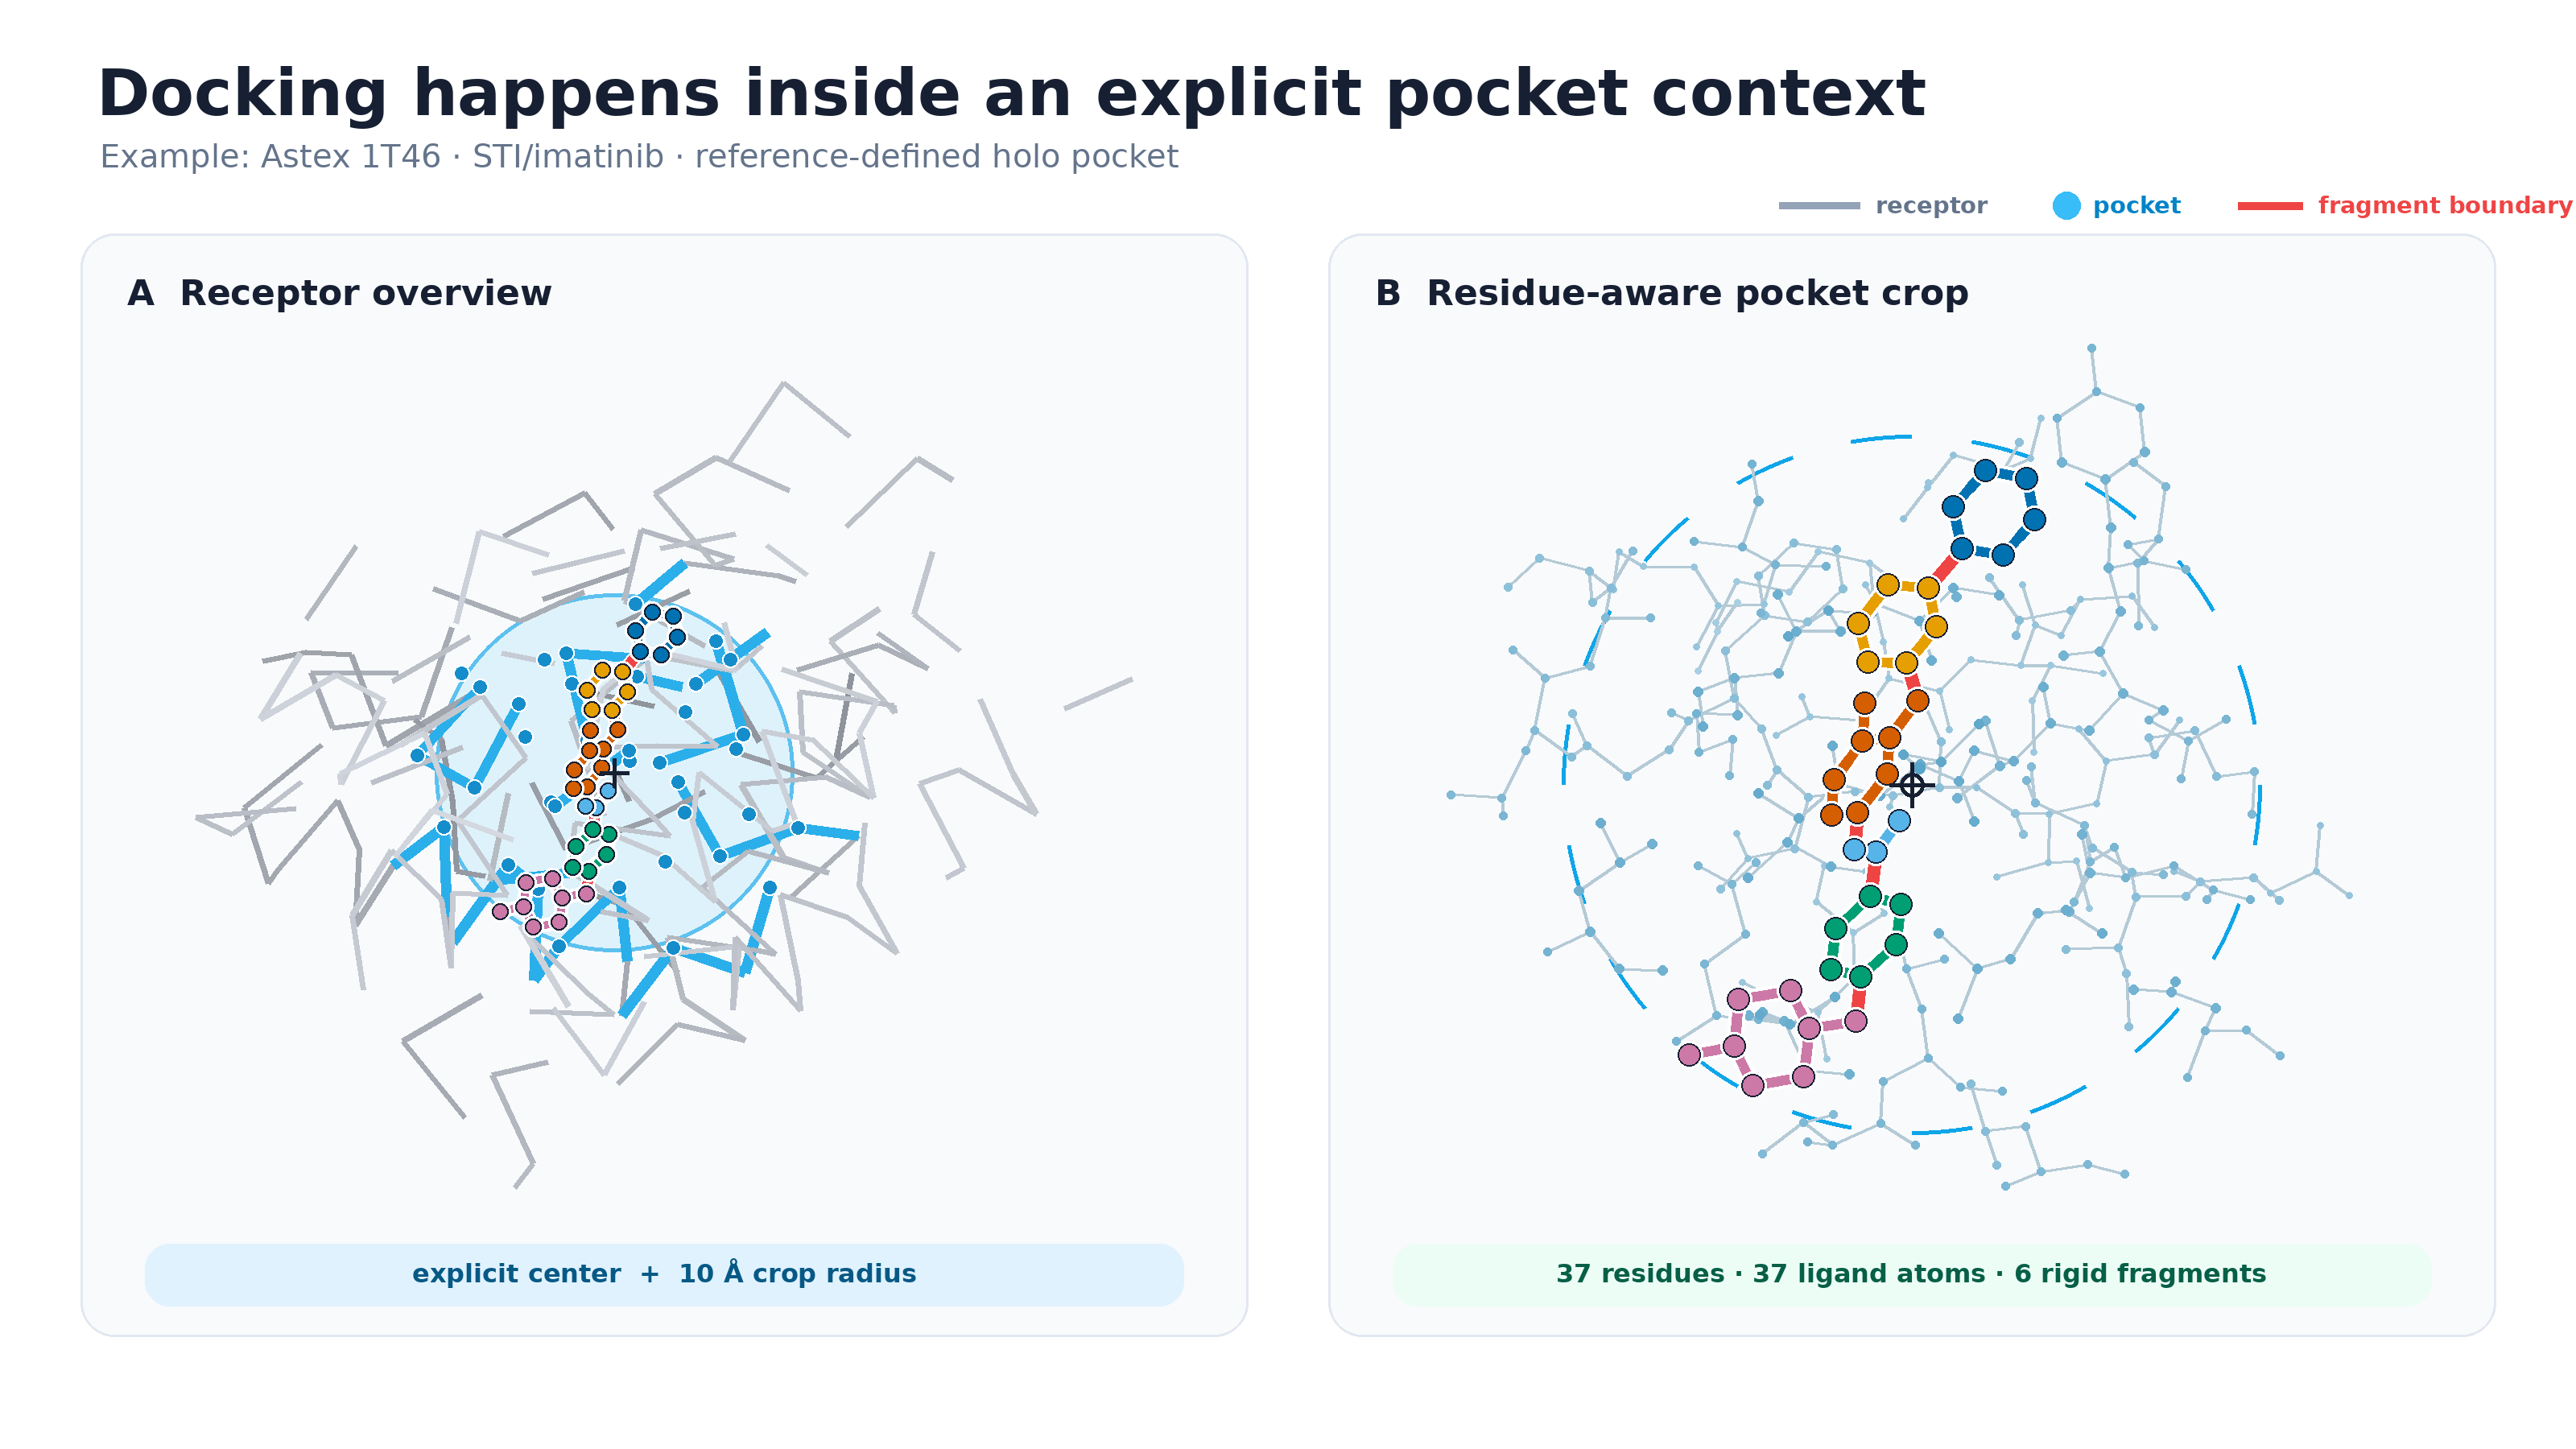
\includegraphics[width=\textwidth]{protein_pocket_context.png}
    \caption{Explicit-pocket inference boundary illustrated on Astex 1T46.
    The supplied center defines a residue-aware \(10\,\angstrom\) receptor
    crop. The reference ligand is shown only to explain this diagnostic; it is
    removed before sampling. Because the center is target-derived, the
    experiment measures redocking robustness rather than pocket discovery.}
    \label{fig:pocket_context}
\end{figure}

\subsection{Pocket crop and center perturbation}

We characterize the promoted model under the pre-registered V2
pocket-sensitivity protocol. The docking and
confidence checkpoints, 80-candidate budget, 25-step integrator,
\(\sigma=0.5\,\angstrom\), and per-complex random stream are fixed. We vary
the receptor crop radius over \(\{6,8,10,12\}\,\angstrom\) and perturb each
reference-defined center by isotropic Gaussian noise with standard deviation
\(\{0,1,2\}\,\angstrom\). The 1 and \(2\,\angstrom\) perturbations for one
complex share a direction, enabling within-complex interpretation of the
perturbation magnitude. All 24 dataset--condition runs cover all 85 Astex and
308 PoseBusters complexes without unresolved failures. This study
characterizes robustness only; external benchmark outcomes are not used to
select a new default crop radius.

\subsection{Metrics}

The primary pose metric is top-1 symmetry-aware heavy-atom RMSD success below
\(2\,\angstrom\). We additionally report median RMSD, oracle top-80 success,
failure rate, and official PoseBusters validity excluding the RMSD criterion.
Sampling coverage and top-1 selection are reported separately: an oracle
success is not a deployable docking success. Likewise, a docking score is used
for within-candidate selection and is not interpreted as binding affinity.
For primary complex-level success proportions we report 95\% Wilson intervals
where space permits. These intervals describe finite benchmark-set
uncertainty; they do not replace variability across training or sampling
seeds, which has not yet been measured for the promoted stack.

\section{Results}
\label{sec:results}

\subsection{Frozen reference-pocket redocking}

Table~\ref{tab:frozen_benchmark} summarizes the active frozen-manifest
evaluation. Pure confidence selects 488 poses below \(2\,\angstrom\) among
678 complexes, compared with 483 for Vina+DG and 486 for the historical
composite selector. The corresponding pure-confidence success rates are
76.47\% on Astex (65/85; 95\% Wilson interval 66.43--84.22\%), 73.05\% on
PoseBusters (225/308; 67.84--77.70\%), and 69.47\% on CASF (198/285;
63.90--74.53\%).

\begin{table}[H]
    \centering
    \caption{Top-1 symmetry-aware heavy-atom RMSD \(<2\,\angstrom\) under
    the frozen reference-pocket N80/S25 protocol. Oracle-80 is diagnostic
    only. The composite is retained for historical compatibility, whereas
    pure confidence is the deployable learned selector.}
    \label{tab:frozen_benchmark}
    \begingroup
    \small
    \setlength{\tabcolsep}{3.5pt}
    \begin{tabular}{lrrrrrr}
        \toprule
        Dataset & \(N\) & First (\%) & Vina+DG (\%) & Pure conf. (\%) &
        Frozen comp. (\%) & Oracle-80 (\%) \\
        \midrule
        Astex Diverse & 85  & 32.94 & 77.65 & 76.47 & 78.82 & 95.29 \\
        PoseBusters v2 & 308 & 35.71 & 71.10 & 73.05 & 72.73 & 94.81 \\
        CASF-2016 & 285 & 32.98 & 69.47 & 69.47 & 68.42 & 91.93 \\
        \bottomrule
    \end{tabular}
    \endgroup
\end{table}

The median RMSD of pure-confidence selections is \(1.156\,\angstrom\),
\(1.211\,\angstrom\), and \(1.274\,\angstrom\) on Astex, PoseBusters, and
CASF, respectively. Learned ranking improves over the same-candidate Vina+DG
baseline on PoseBusters but not uniformly across all three datasets. Likewise,
the frozen composite does not dominate pure confidence. These results support
the simpler minimum-predicted-RMSD rule as the deployment default but do not
establish superiority to external docking methods, whose pocket information,
candidate budgets, receptor preparation, and post-processing may differ.

\subsection{Candidate generation and pose selection are distinct bottlenecks}

Oracle-80 success exceeds 91\% on every dataset, leaving gaps of 18.82,
21.76, and 22.46 percentage points between pure-confidence top-1 and oracle
coverage on Astex, PoseBusters, and CASF. Thus most benchmark complexes have a
near-native candidate, but the ranker does not consistently identify it.
The gap is not attributed solely to confidence: the first-pose rates near
33--36\% show that candidate ordering from the stochastic generator is not
itself a useful selection rule.

The retained confidence checkpoint was selected on PLINDER validation rather
than on an external benchmark. On the frozen first 512 validation complexes,
minimum predicted RMSD gives 58.40\% top-1 success and the candidate oracle
gives 77.93\%. Four registered 1,500-step continuation studies---an unchanged
control, setwise, pairwise, and RMSD-listwise training---finish between 57.62
and 58.40\% and none passes the pre-registered \(+1.5\)-point gate. A separate
cluster-free filter changes only 3.72\% of selections on the full 1,076-complex
validation split and improves success from 53.90\% to 54.18\%, below its
\(1.0\)-point deployment gate. We therefore retain the unmodified step-42,500
confidence checkpoint and report the unsuccessful variants rather than
selecting post hoc on the external sets.

\subsection{Pocket context and center error}

Table~\ref{tab:pocket_sensitivity} reports pure-confidence top-1 success in
the separately frozen V2 sensitivity run. With an accurate center, a
\(6\,\angstrom\) crop is 25.88 points below \(10\,\angstrom\) on Astex and
28.57 points below it on PoseBusters. The best accurate-center crop is
\(8\,\angstrom\) for Astex and \(12\,\angstrom\) for PoseBusters, so no
single alternative consistently improves over the \(10\,\angstrom\) matched
default.

\begin{table}[H]
    \centering
    \caption{Pure-confidence top-1 RMSD \(<2\,\angstrom\) (\%) as a function
    of receptor crop radius and Gaussian center perturbation. Each row is one
    full-dataset condition of the promoted N80/S25 stack.}
    \label{tab:pocket_sensitivity}
    \begingroup
    \small
    \setlength{\tabcolsep}{8pt}
    \begin{tabular}{llrrrr}
        \toprule
        Dataset & Center jitter & \(6\,\angstrom\) & \(8\,\angstrom\) &
        \(10\,\angstrom\) & \(12\,\angstrom\) \\
        \midrule
        Astex (\(N=85\)) & \(0\,\angstrom\) & 50.59 & \textbf{77.65} & 76.47 & 76.47 \\
        & \(1\,\angstrom\) & 35.29 & \textbf{67.06} & \textbf{67.06} & \textbf{67.06} \\
        & \(2\,\angstrom\) & 29.41 & \textbf{45.88} & 42.35 & 40.00 \\
        \addlinespace
        PoseBusters (\(N=308\)) & \(0\,\angstrom\) & 44.16 & 66.56 & 72.73 & \textbf{74.03} \\
        & \(1\,\angstrom\) & 39.61 & 53.90 & \textbf{61.04} & 60.71 \\
        & \(2\,\angstrom\) & 20.78 & 31.17 & \textbf{34.42} & 31.17 \\
        \bottomrule
    \end{tabular}
    \endgroup
\end{table}

At the matched \(10\,\angstrom\) crop, \(1\,\angstrom\) center noise reduces
top-1 success from 76.47\% to 67.06\% on Astex and from 72.73\% to 61.04\%
on PoseBusters. At \(2\,\angstrom\), the rates fall to 42.35\% and 34.42\%.
Oracle-80 success at the same crop decreases from 94.12\% to 64.71\% on
Astex and from 93.18\% to 55.52\% on PoseBusters between zero and
\(2\,\angstrom\) perturbation. Center error therefore reduces generator
coverage, not only confidence ranking. Because this is an external-set
characterization, it does not by itself authorize changing the
\(10\,\angstrom\) inference default.

\subsection{Performance degrades for large and flexible ligands}

The same-candidate slices identify ligand size and flexibility as major failure
axes. On PoseBusters, pure-confidence success is 78.33\% for ligands with at
most 20 heavy atoms (\(N=120\)) but 44.00\% above 40 heavy atoms (\(N=25\));
oracle coverage decreases from 99.17\% to 60.00\%. For ligands with at least
eight rotatable bonds (\(N=66\)), pure-confidence and oracle success are
62.12\% and 86.36\%, compared with 77.88\% and 98.23\% for at most three
rotatable bonds (\(N=113\)). CASF shows the same size trend: pure-confidence
success drops from 82.57\% at at most 20 heavy atoms (\(N=109\)) to 38.89\%
above 40 atoms (\(N=18\)), with oracle coverage dropping from 97.25\% to
55.56\%. These paired declines indicate that larger ligands stress both
fragment-pose generation and candidate selection.

\subsection{Pose accuracy does not guarantee physical validity}

Official PoseBusters evaluation is currently available for the frozen
composite-selected poses, not for the pure-confidence selections. It gives a
pass-all rate of 54.87\% (169/308) when the RMSD criterion is excluded,
substantially below the corresponding composite RMSD success of 72.73\%.
Protein minimum-distance and tetrahedral-chirality checks pass for 69.16\% and
78.25\% of complexes, respectively, whereas internal clash, energy,
bond-length, and bond-angle checks each exceed 95\%. Near-native placement and
physical/chemical validity are therefore distinct failure axes.

A registered inference-only Vina-guidance study provides a negative result.
Guidance raises composite-selected official validity from 54.87\% to 56.17\%
without changing top-1 RMSD success, but the paired gain is only 1.30
percentage points (95\% bootstrap interval \(-0.32\) to \(3.25\) points;
exact McNemar \(p=0.289\)). It does not meet the pre-registered \(+3\)-point
validity target and is not included in the promoted default.

\section{Discussion and Limitations}
\label{sec:discussion}

\method separates three sources of docking performance: candidate generation,
within-set selection, and molecular validity. High oracle-80 coverage indicates
that the fragment-level flow often reaches the native basin, whereas the
smaller top-1 rates quantify a ranking gap. The PoseBusters validity result
shows a second, partly independent gap that cannot be inferred from RMSD alone.
Registered selector and guidance studies did not pass their deployment gates,
which argues against attributing the remaining gap to a single post-processing
choice.

The rigid-fragment state reduces the dimensionality of ligand motion and
preserves within-fragment geometry, but independent fragment motions can still
distort cut-bond geometry or create protein clashes. The auxiliary atom and
distance-geometry losses mitigate these effects without enforcing a complete
molecular mechanics model. Large and highly flexible ligands remain the
clearest observed failure regime. Their lower oracle coverage shows that
improving only the confidence model will not resolve this weakness.

The pocket study further distinguishes receptor context from pocket
localization. Crops below \(8\,\angstrom\) remove useful receptor information,
whereas modest differences among \(8\), \(10\), and \(12\,\angstrom\) depend
on the dataset. In contrast, a \(2\,\angstrom\) center perturbation sharply
reduces both top-1 and oracle success. Robust deployment therefore requires an
independently validated pocket definition; random crop augmentation during
training does not make the model insensitive to localization error.

The present evaluation is reference-pocket redocking with a rigid receptor.
It does not test blind site identification, apo-to-holo receptor changes,
induced fit, affinity prediction, virtual screening, covalent docking, or
prospective generalization. In addition, the currently preserved training
split is a compatibility asset rather than the final strict external-exclusion
split. These limitations constrain the claims that can be made from the
current results. Literature values obtained with different pocket inputs,
candidate budgets, receptor preparation, or post-processing are therefore not
used as matched baselines in the main table.

The highest-priority next evidence is a strict ligand- and pocket-disjoint
training split with frozen external exclusions, followed by matched reruns of
representative classical and learned baselines. Independent training or
sampling seeds, wall-clock and memory measurements, and component ablations
for fragmentation, Newton--Euler aggregation, and auxiliary geometry losses
are also required to isolate which design choices cause the observed behavior.
Target-independent pocket centers and apo or predicted receptors would extend
the evidence beyond the present holo redocking boundary.

\section{Conclusion}
\label{sec:conclusion}

We presented \method, a fragment-based \(\SE(3)\)-equivariant flow-matching
framework for pocket-conditioned protein--ligand docking. The method combines
a unified atom--fragment--protein graph, an equivariant atom-force head,
Newton--Euler fragment dynamics, and a separately trained confidence ranker.
Across three frozen reference-pocket diagnostics, the promoted stack places a
near-native candidate among 80 samples for 91.93--95.29\% of complexes and
selects one as top-1 for 69.47--76.47\%. Robustness and slice analyses show
that pocket-center error, ligand size, and flexibility reduce generator
coverage as well as ranking accuracy, while the PoseBusters checks reveal a
separate molecular-validity gap. These results establish the behavior of the
current pocket-conditioned system without claiming blind or prospective
docking. A submission-level evaluation should next combine a strictly
leakage-controlled split, target-independent pocket definitions, matched
baselines, component ablations, and compute measurements.

\section*{Data and Code Availability}

The manuscript is accompanied by configuration files, checkpoint manifests,
evaluation protocols, and scripts that define the reported EFF-Dock
workflows. Raw PLINDER and external benchmark structures remain subject to
their original licenses and distribution terms.
\todo{Before submission, insert the permanent public repository URL, release
tag, archival DOI, and exact instructions for obtaining each raw dataset.}

\section*{Author Contributions}

J.S. and J.L. conceived the study and designed the experiments. J.S.
implemented the models, performed the experiments, and analyzed the results.
J.S. and J.L. interpreted the findings and wrote the manuscript. J.L.
supervised the study.

\section*{Supporting Information}

The Supporting Information contains detailed node and edge construction,
equivariant normalization and aggregation, the Newton--Euler observable
subspace, auxiliary objectives, confidence-model targets and losses, and
additional reproducibility material.

\section*{Acknowledgments}

\todo{Insert all funding agencies and grant numbers, computing-resource
acknowledgments, and any venue-required disclosure of writing or coding tools.}

\section*{Competing Interests}

\todo{Confirm the final competing-interest statement, including whether the
Arontier affiliation requires a specific disclosure for this work.}


\bibliographystyle{plainnat}
\bibliography{references}

\appendix
\section{Architecture and Objective Details}
\label{app:architecture_details}

This appendix specifies the implementation-level equations omitted from the
main text. All distances supplied to neural networks are represented by their
numerical values in Angstrom.

\subsection{Node initialization and edge features}
\label{app:edge_features}

\paragraph{Radial basis.}
For an edge distance \(d\), the docking trunk uses 32 Gaussian radial basis
functions
\begin{equation}
    \rho_m(d)
    =
    \exp\left[-\frac{(d-\mu_m)^2}{2\Delta^2}\right],
    \qquad
    \mu_m\in[0,16]\,\angstrom,\quad
    \Delta=\frac{16}{32}\,\angstrom.
    \label{eq:rbf}
\end{equation}

\paragraph{Conditioning and initialization.}
The conditioning vector in Eq.~\eqref{eq:time_sigma_embedding} uses a
32-dimensional sinusoidal embedding. The final linear map of the prior-scale
branch is initialized to zero. Let \(\mathbf{a}_i\) denote raw node
attributes. Initial scalar states are
\begin{align}
    \mathbf{s}^{0}_i
    &=
    \operatorname{MLP}_{\mathrm{node}}(\mathbf{a}_i),
    \qquad i\notin\mathcal{V}_{\mathrm{frag}},\\
    \mathbf{s}^{0}_k
    &=
    \operatorname{MLP}_{\mathrm{frag}}
    \left(
      \left[
      \operatorname{MLP}_{\mathrm{node}}(\mathbf{a}_k),
      \operatorname{Emb}(|\mathcal{A}_k|),
      \boldsymbol{\eta}_{b(k)}
      \right]
    \right),
    \qquad k\in\mathcal{V}_{\mathrm{frag}}.
    \label{eq:scalar_initialization}
\end{align}
With graph center
\(\mathbf{c}_b=|\mathcal{V}_b|^{-1}\sum_{i\in\mathcal{V}_b}\mathbf{x}_i\),
the \(c\)-th initial \(1o\) channel is
\begin{equation}
    \mathbf{h}^{0,1o}_{i,c}
    =
    G_c(\mathbf{s}^{0}_i)(\mathbf{x}_i-\mathbf{c}_{b(i)})
    +
    \mathbb{1}_{i\in\mathcal{V}_{\mathrm{frag}}}
    \sum_{q=1}^{3}W^{R}_{cq}\mathbf{R}_{i,t}^{(:,q)}.
    \label{eq:vector_initialization}
\end{equation}
Here \(G_c\) ends in \(\tanh\), \(\mathbf{R}^{(:,q)}\) is a rotation-matrix
column, and \(W^R\) is zero-initialized.

\paragraph{Complete edge scalar.}
Let \(\bar{\mathbf{s}}_i^{(\ell)}\in\R^{384}\) be the scalar block after
pre-normalization. The reference-distance feature is
\begin{equation}
    \boldsymbol{\delta}_{ji}
    =
    \left[
      d_{ji},\;
      d_{ji}-d^{\mathrm{ref}}_{ji},\;
      q_{ji}\log
      \frac{d_{ji}}{d^{\mathrm{ref}}_{ji}+\epsilon},\;
      q_{ji}
    \right],
    \qquad
    q_{ji}=\mathbb{1}[d^{\mathrm{ref}}_{ji}>0].
    \label{eq:distance_evolution}
\end{equation}
For a source assigned to fragment \(k\), the local-frame feature is
\(\mathbf{R}_{k,t}^{\top}\mathbf{r}_{ji}\); it is zero otherwise. The
six-dimensional pair vector \(\boldsymbol{\chi}_{ji}\) represents
hydrogen-bond compatibility, salt-bridge compatibility, equal-charge clash,
hydrophobic contact, halogen--acceptor contact, and metal coordination. The
full edge descriptor is
\begin{align}
    \mathbf{e}^{(\ell)}_{ji}
    =\big[
      &\boldsymbol{\rho}(d_{ji}),
      \operatorname{Emb}(\tau_{ji}),
      \operatorname{Emb}(\mathrm{bond}_{ji}),
      W_d\boldsymbol{\delta}_{ji},
      \operatorname{Emb}(\mathrm{hop}_{ji}),\nonumber\\
      &W_R\mathbf{R}_{k,t}^{\top}\mathbf{r}_{ji},
      W_c\boldsymbol{\chi}_{ji},
      \bar{\mathbf{s}}_j^{(\ell)},
      \bar{\mathbf{s}}_i^{(\ell)},
      \boldsymbol{\eta}_{b(i)}
    \big]\in\R^{1020}.
    \label{eq:edge_scalar}
\end{align}
The bond embedding concatenates bond order, conjugation, ring, and
stereochemistry embeddings; unavailable attributes use explicit sentinel
categories.

\subsection{Equivariant normalization and gated aggregation}

\paragraph{Normalization and activation.}
For an \((l,p)\) block
\(\mathbf{h}^{lp}\in\R^{C_{lp}\times(2l+1)}\), equivariant RMS
normalization is
\begin{align}
    \operatorname{rms}_{lp}(\mathbf{h})
    &=
    \left(
      \frac{1}{C_{lp}}
      \sum_{c=1}^{C_{lp}}\|\mathbf{h}^{lp}_c\|_2^2+\epsilon
    \right)^{1/2},\\
    \operatorname{RMSNorm}(\mathbf{h})^{lp}_c
    &=
    \gamma^{lp}_c
    \frac{\mathbf{h}^{lp}_c}{\operatorname{rms}_{lp}(\mathbf{h})}.
    \label{eq:irrep_rmsnorm}
\end{align}
\(0e\) scalars receive SiLU. Non-scalar channels receive invariant norm gates,
\begin{equation}
    \operatorname{EqAct}(\mathbf{h})^{lp}_c
    =
    \mathbf{h}^{lp}_c\,
    \operatorname{sigmoid}
    \left(
      A^{lp}_c(
      \{\|\mathbf{h}^{l'p'}_{c'}\|_2\}_{l'>0,c'})
    \right),
    \qquad l>0.
    \label{eq:equivariant_activation}
\end{equation}
Dropout samples one mask per irrep channel and broadcasts it over the
\(2l+1\) representation components.

\paragraph{Dual radial scales.}
The input and output channel scales in Eq.~\eqref{eq:tp_message} are
\begin{equation}
    \mathbf{u}_{ji}^{(\ell)}
    =
    \operatorname{SiLU}
    (W_r^{(\ell)}\mathbf{e}_{ji}^{(\ell)}+\mathbf{b}_r^{(\ell)}),
    \qquad
    \boldsymbol{\alpha}_{ji}^{\mathrm{in/out}}
    =
    \mathbf{1}
    +W_{\mathrm{in/out}}^{(\ell)}
    \mathbf{u}_{ji}^{(\ell)}.
    \label{eq:dual_radial}
\end{equation}
The scales are broadcast across all \(2l+1\) components of a channel.

\paragraph{Edge gates and aggregation.}
For edge type \(\tau_{ji}\), the gate network returns a scalar component and
one component per non-scalar channel:
\begin{align}
    [a_{ji}^{0},\mathbf{a}_{ji}^{\mathrm{ns}}]
    &=
    \operatorname{MLP}_{g}^{(\ell)}
    (\mathbf{e}_{ji}^{(\ell)}),\\
    g_{ji}^{0}
    &=
    \operatorname{sigmoid}(a_{ji}^{0})
    \exp\left(-\frac{d_{ji}}{\zeta_{\tau_{ji}}^{(\ell)}}\right),
    \qquad
    \zeta_{\tau,\mathrm{init}}^{(\ell)}=8\,\angstrom,\\
    g_{ji,c}^{lp}
    &=
    g_{ji}^{0}\operatorname{sigmoid}(a_{ji,c}^{lp}),
    \qquad l>0.
    \label{eq:edge_gates}
\end{align}
Scalar and non-scalar aggregates are respectively
\begin{align}
    \mathbf{q}_{i,c}^{0e}
    &=
    \frac{
      \sum_{j\in\mathcal{N}(i)}
      g_{ji}^{0}\mathbf{m}_{ji,c}^{0e}
    }{
      \sum_{j\in\mathcal{N}(i)}g_{ji}^{0}+\epsilon
    },
    \label{eq:scalar_aggregation}\\
    \widetilde{\mathbf{q}}_{i,c}^{lp}
    &=
    \frac{
      \sum_{j\in\mathcal{N}(i)}
      g_{ji,c}^{lp}\mathbf{m}_{ji,c}^{lp}
    }{
      \sum_{j\in\mathcal{N}(i)}g_{ji,c}^{lp}+\epsilon
    }.
    \label{eq:nonscalar_aggregation}
\end{align}
Channels with the same \(l\) are split into direction and magnitude. If
\(\boldsymbol{\nu}_{i,l}\) concatenates
\(\|\widetilde{\mathbf{q}}_{i,c}^{lp}\|_2\) across both parities, then
\begin{equation}
    \mathbf{q}_{i,c}^{lp}
    =
    \frac{\widetilde{\mathbf{q}}_{i,c}^{lp}}
         {\|\widetilde{\mathbf{q}}_{i,c}^{lp}\|_2+\epsilon}
    \left[
      \operatorname{SiLU}
      (W_l^{(\ell)}\boldsymbol{\nu}_{i,l}+\mathbf{b}_l^{(\ell)})
    \right]_c.
    \label{eq:nonscalar_rescale}
\end{equation}

\paragraph{Adaptive normalization.}
Let
\(\mathbf{u}_i^{(\ell)}
=\mathbf{h}_i^{(\ell)}
+\operatorname{EqBlock}^{(\ell)}(\mathbf{q}_i^{(\ell)})\) and
\(\bar{\mathbf{u}}=\operatorname{RMSNorm}(\mathbf{u})\). The expanded form of
Eq.~\eqref{eq:compact_layer_update} is
\begin{align}
    \mathbf{h}_{i}^{(\ell+1),0e}
    &=
    \bar{\mathbf{u}}_{i}^{0e}
    \odot(\mathbf{1}+\boldsymbol{\gamma}_{i}^{0e})
    +\boldsymbol{\beta}_{i}^{0e},\\
    \mathbf{h}_{i,c}^{(\ell+1),lp}
    &=
    \bar{\mathbf{u}}_{i,c}^{lp}
    \left[1+0.1\tanh(\gamma_{i,c}^{lp})\right],
    \qquad l>0,\\
    [\boldsymbol{\gamma}_{i}^{0e},
      \boldsymbol{\beta}_{i}^{0e},
      \boldsymbol{\gamma}_{i}^{\mathrm{ns}}]
    &=
    W_{\eta}^{(\ell)}\boldsymbol{\eta}_{b(i)}
    +\mathbf{b}_{\eta}^{(\ell)}.
    \label{eq:equivariant_adaln}
\end{align}
The conditioning projection is zero-initialized.

\subsection{Newton--Euler observable subspace}
\label{app:newton_euler_details}

For
\(\mathbf{I}_k=\mathbf{V}_k
\operatorname{diag}(\boldsymbol{\lambda}_k)\mathbf{V}_k^\top\), define
\begin{align}
    m_{ka}
    &=
    \mathbb{1}[|\mathcal{A}_k|>1]\,
    \mathbb{1}
    \left[
      \lambda_{ka}>0.01\max_b\lambda_{kb}
    \right],\\
    \mathbf{I}_k^{+}
    &=
    \mathbf{V}_k
    \operatorname{diag}
    \left(
      \frac{m_{ka}}{\max(\lambda_{ka},10^{-6})}
    \right)
    \mathbf{V}_k^\top,\\
    \mathbf{P}_k
    &=
    \mathbf{V}_k\operatorname{diag}(\mathbf{m}_k)\mathbf{V}_k^\top.
    \label{eq:observable_projection}
\end{align}
The eigendecomposition is evaluated on a symmetrized double-precision inertia
matrix. Single-atom fragments bypass the eigensolver.

\subsection{Auxiliary docking losses}
\label{app:loss_details}

The atom-level auxiliary objective is
\begin{align}
    \widehat{\mathbf{u}}_i
    &=
    \widehat{\mathbf{v}}_{g(i)}
    +
    \widehat{\boldsymbol{\omega}}_{g(i)}
    \times\mathbf{r}_i,\\
    \mathbf{u}^{\star}_i
    &=
    \mathbf{v}^{\star}_{g(i)}
    +
    \boldsymbol{\omega}^{\star}_{g(i)}
    \times\mathbf{r}_i,\\
    \mathcal{L}_{\mathrm{atom}}
    &=
    \frac{1}{3N}
    \sum_{i=1}^{N}
    \|\widehat{\mathbf{u}}_i-\mathbf{u}^{\star}_i\|_2^2.
    \label{eq:atom_aux_loss}
\end{align}

For the distance-geometry loss, one predicted step gives
\begin{align}
    \widetilde{\mathbf{T}}_{k,1}
    &=
    \mathbf{T}_{k,t_b}
    +(1-t_b)\widehat{\mathbf{v}}_k,\\
    \widetilde{\mathbf{R}}_{k,1}
    &=
    \operatorname{Exp}
    \left((1-t_b)\widehat{\boldsymbol{\omega}}_k\right)
    \mathbf{R}_{k,t_b},\\
    \widetilde{\mathbf{x}}_{i,1}
    &=
    \widetilde{\mathbf{R}}_{g(i),1}\mathbf{y}_i
    +\widetilde{\mathbf{T}}_{g(i),1}.
    \label{eq:one_step_endpoint}
\end{align}
For inter-fragment atom pairs
\(\mathcal{P}_b=\{(i,j):i<j,\ g(i)\neq g(j)\}\),
\begin{equation}
    \mathcal{L}_{\mathrm{DG}}
    =
    \frac{
      \sum_b t_b^2
      \frac{1}{|\mathcal{P}_b|}
      \sum_{(i,j)\in\mathcal{P}_b}
      \left(
        \|\widetilde{\mathbf{x}}_{i,1}
          -\widetilde{\mathbf{x}}_{j,1}\|_2
        -
        \|\mathbf{x}^{\star}_i-\mathbf{x}^{\star}_j\|_2
      \right)^2
    }{
      \sum_b t_b^2
    }.
    \label{eq:distance_geometry_loss}
\end{equation}

\section{Confidence Model Details}
\label{app:confidence_details}

\subsection{Invariant features and readout}

For candidate \(m\), the confidence hidden state is initialized by
\begin{equation}
    \mathbf{h}^{C,0}_{mi}
    =
    \mathbf{h}^{\mathrm{fresh}}_{mi}
    +
    \alpha\,
    \mathbb{1}
    [i\in\mathcal{V}_{\mathrm{lig\text{-}atom}}
      \cup\mathcal{V}_{\mathrm{frag}}]\,
    \mathbf{h}^{D}_{mi},
    \qquad \alpha_{\mathrm{init}}=0.25.
    \label{eq:confidence_hidden_init}
\end{equation}
The invariantized node descriptor is
\begin{equation}
    \mathbf{z}_{mi}
    =
    \left[
      \mathbf{h}_{mi}^{0e},
      \{\|\mathbf{h}_{mi,c}^{lp}\|_2\}_{l>0,p,c}
    \right].
    \label{eq:confidence_invariants}
\end{equation}

For ligand atom \(i\), let
\(d_{mip}=\|\mathbf{x}_{mi}-\mathbf{x}_p\|_2\),
\(d^{\min}_{mi}=\min_p d_{mip}\), and
\(w_{mip}=\exp[-d_{mip}/(2\,\angstrom)]\). With protein-atom flags
\(\mathbf{q}_p\), the explicit contact descriptor is
\begin{align}
    \mathbf{c}_{mi}
    =\bigg[
      &\frac{d^{\min}_{mi}}{10\,\angstrom},
      \boldsymbol{\rho}_{[0,10]}(d^{\min}_{mi}),
      \left\{
      \log\left(1+\sum_p\mathbb{1}[d_{mip}<r]\right)
      \right\}_{r\in\{2,3.5,5\}\,\angstrom},\nonumber\\
      &\log\left(1+\sum_p w_{mip}\right),
      \frac{\sum_p w_{mip}\mathbf{q}_p}
           {\sum_p w_{mip}+\epsilon}
    \bigg].
    \label{eq:confidence_contact_features}
\end{align}
The atom features and outputs are
\begin{align}
    \mathbf{a}_{mi}
    &=
    \operatorname{MLP}_{a}
    \left(
      \operatorname{LN}[
      \mathbf{z}_{mi},\mathbf{c}_{mi}]
    \right),\\
    [\widehat{\ell}^{\,\mathrm{atom}}_{mi},
      \widehat{o}^{\,\mathrm{atom}}_{mi}]
    &=
    \operatorname{MLP}_{\mathrm{atom}}(\mathbf{a}_{mi}).
    \label{eq:confidence_atom_head}
\end{align}

Contact attention is
\begin{align}
    \mathbf{u}_{mi}
    &=
    \operatorname{MLP}_{c}
    \left(
      \operatorname{LN}[
      \mathbf{a}_{mi},\mathbf{c}_{mi}]
    \right),\\
    \alpha_{mi}
    &=
    \frac{
      \exp(s(\mathbf{u}_{mi}))
    }{
      \sum_{j\in\mathcal{V}_{\mathrm{lig\text{-}atom}}}
      \exp(s(\mathbf{u}_{mj}))
    },\\
    \mathbf{r}^{\mathrm{contact}}_m
    &=
    \left[
      \sum_i\alpha_{mi}\mathbf{u}_{mi},
      \max_i\mathbf{u}_{mi},
      \operatorname{mean}_i\mathbf{a}_{mi},
      \max_i\mathbf{a}_{mi}
    \right].
    \label{eq:contact_attention}
\end{align}
For node type
\(q\in\{\mathrm{lig\text{-}atom},\mathrm{frag},
\mathrm{prot\text{-}atom},\mathrm{prot\text{-}res}\}\), let
\(\mathbf{v}_{mi}=\operatorname{MLP}_g(\operatorname{LN}(\mathbf{z}_{mi}))\).
Then
\begin{equation}
    \mathbf{r}^{\mathrm{global}}_m
    =
    \mathop{\Vert}_{q}
    \left[
      \operatorname{mean}_{i:\tau(i)=q}\mathbf{v}_{mi},
      \max_{i:\tau(i)=q}\mathbf{v}_{mi}
    \right].
    \label{eq:global_type_pooling}
\end{equation}
The pose head is defined in Eq.~\eqref{eq:confidence_pose_head}; its reported
RMSD prediction is
\begin{equation}
    \widehat{r}_m
    =
    \max
    \left\{
      0,\,
      \exp\left(
        \operatorname{clip}
        (\widehat{\ell}^{\,\mathrm{pose}}_m,-2,5)
      \right)-1
    \right\}.
\end{equation}

\subsection{Confidence targets and losses}
\label{app:confidence_loss_details}

For fixed atom correspondence,
\begin{equation}
    d_{mi}^{\star}
    =
    \|\mathbf{x}_{mi}-\mathbf{x}^{\star}_i\|_2,
    \qquad
    r_m^{\star}
    =
    \left(
      \frac{1}{N}\sum_i(d_{mi}^{\star})^2
    \right)^{1/2}.
    \label{eq:confidence_targets}
\end{equation}
With unit-transition Huber loss \(H_1\) and binary cross entropy
\(\operatorname{BCE}\), the pointwise terms are
\begin{align}
    \mathcal{L}_{\mathrm{atom\text{-}reg}}
    &=
    \frac{1}{MN}\sum_{m,i}
    H_1\left(
      \widehat{\ell}^{\,\mathrm{atom}}_{mi},
      \log(1+d_{mi}^{\star})
    \right),\\
    \mathcal{L}_{\mathrm{pose\text{-}reg}}
    &=
    \frac{1}{M}\sum_m
    H_1\left(
      \widehat{\ell}^{\,\mathrm{pose}}_m,
      \log(1+r_m^{\star})
    \right),\\
    \mathcal{L}_{\mathrm{atom\text{-}BCE}}
    &=
    \frac{1}{MN}\sum_{m,i}
    \operatorname{BCE}
    \left(
      \widehat{o}^{\,\mathrm{atom}}_{mi},
      \mathbb{1}[d_{mi}^{\star}<2\,\angstrom]
    \right),\\
    \mathcal{L}_{\mathrm{pose\text{-}BCE}}
    &=
    \frac{1}{M}\sum_m
    \operatorname{BCE}
    \left(
      \widehat{o}^{\,\mathrm{pose}}_m,
      \mathbb{1}[r_m^{\star}<2\,\angstrom]
    \right).
    \label{eq:confidence_pointwise_losses}
\end{align}

For
\(\mathcal{Q}=\{(m,n):
\log(1+r_n^{\star})-\log(1+r_m^{\star})>0.3\}\), the pairwise term is
\begin{equation}
    \mathcal{L}_{\mathrm{rank}}
    =
    \frac{1}{|\mathcal{Q}|}
    \sum_{(m,n)\in\mathcal{Q}}
    \max
    \left(
      0,\,
      0.05-
      (\widehat{\ell}^{\,\mathrm{pose}}_n
       -\widehat{\ell}^{\,\mathrm{pose}}_m)
    \right),
    \label{eq:confidence_pairwise}
\end{equation}
with zero contribution when \(\mathcal{Q}\) is empty. The success-listwise
target and loss are
\begin{align}
    q_m
    &=
    \frac{
      \operatorname{sigmoid}
      ((2-r_m^{\star})/0.2)
    }{
      \sum_n
      \operatorname{sigmoid}
      ((2-r_n^{\star})/0.2)
    },\\
    \mathcal{L}_{\mathrm{success\text{-}listwise}}
    &=
    -\sum_m q_m
    \log
    \frac{
      \exp(\widehat{o}^{\,\mathrm{pose}}_m)
    }{
      \sum_n\exp(\widehat{o}^{\,\mathrm{pose}}_n)
    }.
    \label{eq:confidence_listwise}
\end{align}

\section{Additional Reproducibility Material}

The active benchmark and sensitivity studies use the promoted geometry
checkpoint at step 100,000 (SHA-256 prefix \texttt{6932fb3ba6eb}) and
confidence checkpoint at step 42,500 (prefix \texttt{e31fde6f3512}). The
training-configuration hash begins with \texttt{39aa62e4a48e}. Full
checkpoint, configuration, and dataset-manifest hashes are retained in the
machine-readable benchmark summaries rather than abbreviated during
execution.

The active runs used PyTorch 2.10.0, CUDA 13.0, and RTX 6000 Ada or H100 PCIe
accelerators. Every final benchmark and pocket-sensitivity condition contains
all frozen IDs with zero unresolved failures. Exact wall-clock and peak-memory
measurements remain to be collected under one dedicated hardware
configuration.

Machine-readable summaries retain the first, Vina+DG, pure-confidence,
historical-composite, and oracle selectors; RMSD thresholds at 1, 2, 3, and
\(5\,\angstrom\); heavy-atom, fragment-count, rotatable-bond, and cofactor
slices; failure and rescue records; runtime versions; and output paths. The
public archival location for these artifacts will be added with the final
code and weight release.


\end{document}
